\bookchapter{פרק 60: הקמת סביבת הפיתוח — Xcode והפרויקט הראשון}

\chapterintro{לפני שעושים את המלאכה, מחדדים את הכלים. בפרק הזה נקים את “המטבח”: נתקין את Xcode, נריץ בהצלחה את המדמה, ניצור את פרויקט ה-iOS הראשון שלכם בחיים, ואז נפרק את מבנה הפרויקט ונבין אותו לעומק. אחרי שהסביבה מוכנה, תראו בפעם הראשונה את הקוד שכתבתם הופך לכפתור שאפשר ללחוץ עליו — רגע שהרבה אנשים זוכרים כל החיים.}

\booksection{מכינים מק}

קודם כל המחסום: פיתוח ל-iOS חייב להתבצע על macOS. אין לכם מק? יש שלוש אפשרויות: לקנות אחד (גם Mac mini או MacBook Air מיד שנייה מספיקים לגמרי), לשכור מק בענן לטווח קצר, או להתחיל קודם בחלק השמיני “פיתוח מעשי ל-Android” (אפשר גם מ-Windows).

\begin{center}
\begin{tabularx}{\linewidth}{|X|X|X|}
\hline
\textbf{הגדרה} & \textbf{דרישה מינימלית} & \textbf{קו נוח (מומלץ)} \tabularnewline
\hline
מעבד & Apple Silicon (מ-M1 ומעלה) & M2 וחדשים יותר \tabularnewline
זיכרון (RAM) & 8GB & 16GB \tabularnewline
דיסק & להשאיר 40GB ומעלה (Xcode עצמו אחד שמן במיוחד) & 256GB ומעלה \tabularnewline
מערכת & macOS העדכני ביותר & להשאיר עדכונים אוטומטיים \tabularnewline
\hline
\end{tabularx}
\end{center}

\begin{center}\small\color{gray}הגדרות ייחוס למחשב פיתוח מק (אוגוסט 2026)\end{center}

\begin{tcbinfo}{טיפ: אפשר ללמוד את השפה גם בלי מק}
Swift Playgrounds החינמי ב-iPad מאפשר ללמוד את יסודות שפת Swift (בלי מק); אפשר להתקין אותו גם ב-iPhone. שחקו קודם עם חומר השפה של פרק 61 ב-Playgrounds עד שיהיה לכם בקצה האצבעות, וכשתקבלו מק — תמריאו ישר. “חידוד הגרזן לא גוזל מזמן הכריתה” — זה בדיוק העניין.

\end{tcbinfo}

\booksection{מתקינים את Xcode}

Xcode היא סביבת הפיתוח המשולבת הרשמית של אפל, והיא חינמית. התקנה בשלושה צעדים:

\begin{enumerate}
  \item במק פתחו את ה-App Store, חפשו "Xcode" ולחצו על התקנה — שימו לב שמדובר בכמה GB, בחרו שעה עם רשת מהירה;
  \item בהפעלה הראשונה אחרי ההתקנה אשרו את הרישיון והשלימו התקנת רכיבים (מתבצע אוטומטית);
  \item בתפריט Xcode Settings Locations ודאו ש-Command Line Tools נבחר — כלי שורת הפקודה הם תנאי מוקדם להרבה סקריפטים וכלים של צד שלישי.
\end{enumerate}

\begin{tcbwarn}{שימו לב: "משחק ההתאמה" בין גרסאות למערכת}
Xcode חדש דורש לרוב את macOS העדכני ביותר, ומק ישן עלול להיתקע בגרסה ישנה. בעלייה ל-App Store אפל מחייבת בנייה ב-Xcode חדש יחסית (בדרך כלל ניתנת תקופת חסד). לכן אל תדחו עדכוני מערכת יותר מדי — מפתחי iOS הם מהקבוצות שדוהרות אחרי גרסאות חדשות בלהט הרב ביותר.

\end{tcbwarn}

\booksection{יוצרים את הפרויקט הראשון שלכם}

פתחו Xcode Create New Project בחרו iOS תבנית App, ואז מלאו:

\begin{center}
\begin{tabularx}{\linewidth}{|X|X|X|}
\hline
\textbf{הגדרה} & \textbf{מה ממלאים} & \textbf{הסבר} \tabularnewline
\hline
Product Name & MyFirstApp & שם האפליקציה \tabularnewline
Team & ה-Apple ID שלכם (חינם) & לצורך החתימה; חשבון אישי מספיק \tabularnewline
Organization Identifier & com.example & מצורף ל-Product Name ליצירת מזהה החבילה \tabularnewline
Interface & SwiftUI & הפריימוורק הראשי של הספר \tabularnewline
Language & Swift & פשוט מאליו \tabularnewline
\hline
\end{tabularx}
\end{center}

\begin{center}\small\color{gray}חמשת הפרטים למילוי ביצירת פרויקט\end{center}

אחרי לחיצה על Create, Xcode ייצור פרויקט שרץ מיד. בפינה השמאלית העליונה בחרו מדמה (למשל iPhone 17) ולחצו על > להרצה — כעבור מספר שניות יופיע על מסך המדמה חלון עם הכיתוב “Hello, world!”. האפליקציית ה-iOS הראשונה שלכם כבר נולדה.

\booksection{פירוק מבנה הפרויקט: מה תפקידו של כל קובץ}

בצד שמאל נמצא סייר הפרויקט; למתחילים מספיק להכיר את אלה:

\begin{center}
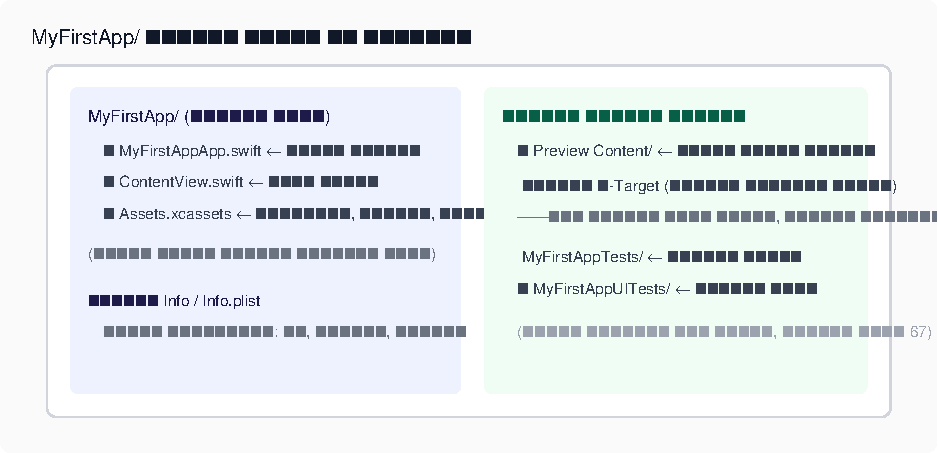
\includegraphics[width=0.92\linewidth]{figures/fig-di-liu-shi-zhang-1}
\\[2pt]\small איור 2: מבנה הפרויקט ב-Xcode שחובה על מתחילים להכיר
\end{center}

\begin{itemize}
  \item MyFirstAppApp.swift: נקודת הכניסה של התוכנה; ב-SwiftUI היא מכילה רק כמה שורות — "התחל, ואז הצג את המסך הראשי";
  \item ContentView.swift: תצוגת המסך הראשי; כל מה שאתם רואים עכשיו נמצא כאן;
  \item Assets.xcassets: מחסן המשאבים — כאן נשמרים האייקונים, התמונות והצבעים;
  \item הגדרות ה-Target: לוחצים על אייקון הפרויקט הכחול בצד שמאל כדי להיכנס; מספר הגרסה, גרסת ה-iOS המינימלית והחתימה — הכול שם. גם את שם התצוגה של האפליקציה ואת האייקון מגדירים כאן.
\end{itemize}

\booksection{ניפוי שגיאות על מכשיר אמיתי: מתקינים את האפליקציה ב-iPhone שלכם}

\booksection{טריקי יעילות ב-Xcode: חמשת “הצ׳יטים” של קיצורי המקשים למתחילים}

ברגע שתשלטו באלה, תיראו “ממש מקצוענים”:

\begin{center}
\begin{tabularx}{\linewidth}{|X|X|X|}
\hline
\textbf{פעולה} & \textbf{קיצור מקשים} & \textbf{מה זה עושה} \tabularnewline
\hline
הרצה & CmdR & מהדר ומריץ \tabularnewline
פתיחה/החלפה של התצוגה המקדימה בקנבס & OptionCmd & המתג של "מה שרואים זה מה שמקבלים" \tabularnewline
עיצוב הזחות & CtrlI & סידור אוטומטי של ההזחה בקוד המסומן \tabularnewline
פתיחת קובץ מהירה & CmdO & מקלידים שם קובץ והוא נפתח מיד (הכי שימושי!) \tabularnewline
הערה/ביטול הערה & Cmd/ & הפעלה וכיבוי מהירים של קוד בזמן ניפוי שגיאות \tabularnewline
\hline
\end{tabularx}
\end{center}

\begin{center}\small\color{gray}קיצורי המקשים השכיחים ב-Xcode (חמישיית המתחילים)\end{center}

עוד שתי הטבות נסתרות: הרצה במקביל של כמה מדמים (להריץ iPhone ו-iPad יחד ולהשוות פריסות) וספריית קטעי קוד (גררו כמה שורות קוד שכיחות אל חלונית ה-Snippets בצד ימין, ופעם הבאה הכניסו אותן בקליק אחד) — תתחילו להשתמש בכלי היעילות, והקלות תגיע מאליה.

\booksection{ניפוי שגיאות על מכשיר אמיתי: מתקינים את האפליקציה ב-iPhone שלכם}

המדמה נהדר, אבל היעד האמיתי הוא מכשיר אמיתי. גם עם Apple ID חינמי אפשר לנפות שגיאות על מכשיר אמיתי:

\begin{enumerate}
  \item חברו את ה-iPhone בכבל נתונים (או נפו שגיאות אלחוטית באותו Wi-Fi);
  \item ברשימת המכשירים למעלה ב-Xcode בחרו את המכשיר שלכם; בפעם הראשונה יתבקשו להתחבר עם Apple ID והחתימה תוגדר אוטומטית;
  \item ב-iPhone: [הגדרות] [כללי] [ניהול VPN ומכשירים] סמכו על תעודת המפתח שלכם;
  \item לחצו על >, והאפליקציה תותקן במכשיר האמיתי.
\end{enumerate}

\begin{tcbwarn}{שימו לב: "מגבלת שבעת הימים" של החשבון החינמי}
אפליקציה שנחתמה עם Apple ID חינמי פגה אחרי 7 ימים (הרצה חוזרת אחת מחדשת את התוקף). זהו מנגנון נגד שימוש לרעה של אפל, ולשלב הלמידה הוא מספיק לגמרי; לחשבון מפתח בתשלום (99 דולר לשנה) אין את המגבלה הזאת — נפרט בפרק 67.

\end{tcbwarn}

\booksection{ניסיון ראשון + עזרה ראשונה לשגיאות נפוצות}

\booksection{ניסיון ראשון + עזרה ראשונה לשגיאות נפוצות}

פתחו את ContentView.swift, החליפו את הטקסט ב-Text(“Hello, world!”) בשם שלכם ולחצו על CmdR להרצה מחדש — כעבור מספר שניות השם שלכם יופיע במדמה. מזל טוב: השלמתם את מחזור “עריכת קוד הידור התקנה הרצה” המלא הראשון שלכם.

\begin{center}
\begin{tabularx}{\linewidth}{|X|X|X|}
\hline
\textbf{תסמין השגיאה} & \textbf{סיבה נפוצה} & \textbf{התרופה} \tabularnewline
\hline
שגיאת Signing & לא נבחר Team או תעודה שפג תוקפה & ב-Target Signing סמנו את החשבון שלכם; בחשבון חינמי פשוט מריצים שוב \tabularnewline
מסך שחור במדמה / הוא לא נפתח & תמונת המערכת פגומה & בתפריט Device Erase All Content; או מוחקים את המדמה ומוסיפים אותו מחדש \tabularnewline
הורדת Xcode איטית / ההתקנה נכשלת & תנודות ברשת של ה-App Store & מנסים בשעה אחרת; או מורידים חבילת .xip להתקנה אופליין מאתר המפתחים של אפל \tabularnewline
\hline
\end{tabularx}
\end{center}

\begin{center}\small\color{gray}טבלת עזרה ראשונה לשגיאות סביבה למתחילים\end{center}

\begin{tcbpractice}{הידיים על ההגה: השלימו את רשימת "טקס הפיתוח" שלכם}
(1) התקינו את Xcode והריצו בהצלחה את המדמה; (2) הריצו את האפליקציה שלכם פעם אחת על מכשיר אמיתי ושמרו צילום מסך למזכרת; (3) החליפו את טקסט ה-Hello בשם שלכם; (4) בהגדרות ה-Target שנו את שם התצוגה של האפליקציה ל“האפליקציה הראשונה שלי”. אחרי ארבעת הצעדים האלה אתם כבר אנשים עם יצירה משלכם.

\end{tcbpractice}

\begin{tcbsummary}{סיכום הפרק}
\begin{itemize}
  \item מחסום קשיח: מק + Xcode; אין מק? למדו את השפה קודם ב-Swift Playgrounds ב-iPad
  \item מתקינים את Xcode מה-App Store; גרסה חדשה דורשת מערכת חדשה — אל תדחו עדכונים
  \item חמשת המרכיבים ביצירת פרויקט חדש: שם, Team, מזהה ארגון, SwiftUI, Swift
  \item כלל אצבע לפרויקט: כל הקוד בתיקיית MyFirstApp/; הגדרות ה-Target מנהלות גרסה וחתימה
  \item ניפוי שגיאות על מכשיר אמיתי עם Apple ID חינמי כולל מגבלת חתימה של 7 ימים; לחשבון בתשלום אין מגבלה כזאת
  \item השגרה היומיומית של המפתח = עריכת קוד CmdR בדיקת התוצאה, שוב ושוב
\end{itemize}

\end{tcbsummary}
